\documentclass[a4paper]{jpconf}
\usepackage{graphicx}
\begin{document}
\title{The CMS Data Aggregation System}

\author{Valentin Kuznetsov}
\address{Cornell University, Ithaca, New York, USA}
\ead{vkuznet@gmail.com}

\author{Dave Evans}
\address{Fermilab, Batavia, Illinois, USA}
\ead{evansde@fnal.gov}

\author{Simon Metson}
\address{Bristol University, Bristol, UK}
\ead{s.metson@bristol.ac.uk}


%In a large modern enterprise, information is almost inevitably distributed among several database management systems. Despite considerable attention from the research community, relatively few commercial systems have attempted to address this issue. This article describes the technology that enables clients of IBM's federated database engine to access and integrate the data and specialized computational capabilities of a wide range of relational and non­relational data sources.

\begin{abstract}
%A meta-data plays significant role in a large modern enterprises, research experiments,
%digital libraries where it comes from different sources and distributed in a 
%variety of forms and digital formats. It is organized and managed by constantly
%evolving software using both relational and non-relational data sources. There is
%a big demand to enable information discovery from multiple sources.
%Here we discuss a new data aggregation system which consume and deliver information 
%from different relational and non-relational data sources on a concrete example 
%of large scale, distributed system of CMS physics experiment at LHC.

Meta-data plays significant role in a large modern enterprises, 
research experiments and digital libraries where it comes from different 
sources and distributed in a variety of forms and digital formats. 
It is organized and managed by constantly evolving software using 
both relational and non-relational data sources. 
Even though we can access it via viriety of data-services, twikies, blogs, etc.,
there is no coherent way for information discovery from different sources
in heterogeneous, distributed environment with different security policies enforced.

Here we discuss a new data aggregation system which consumes, 
indexes and delivers information from different relational and 
non-relational data sources to answer cross data-source queries 
to explore metadata associated to petabytes of experimental data. 
We combine simplpicity of keyword-based search with precision of RDMS
under a new system where aggregated information being collected from various sources 
allowing end-users to place dynamic queries, get precise answers and 
trigger information retrieval on demand. Such close to real-time system 
based on studies  of use cases of the CMS particle physics experiment at 
the LHC which uses a large scale, distributed computing system to motivate the work.

\end{abstract}

\newpage

\section{Introduction}
The CERN, the European Organization for Nuclear Research, plays a leading
role in fundamental studies of physics. It is also known as a place where
World Wide Web was born to help researches share information among each other
via concept of hypertext.
Today, the Large Hadron Collider (LHC) at CERN is marking a new era of High Energy
Physics (HEP), promising to deliver a few PB of data each year. 
At this scale scientists are facing a new set of problems in an area of
``information discovery'' within heterogeneous, distributed environment.
The data and associated meta-data are produced in variety of forms and digital formats.
They are stored into relational and non-releational data-sources, such as 
RDMS systems, document oriented databases, blogs, twikies, customized applications, etc. 
and its access is restricted by broad variety of security policies. 
Working in such environment is not easy and require a lot of knowledge, but users
(in this case physicists) are always looking for simple, intuitive and flexible
tool to look-up their desired data. A well-known solutions, such as web-services,
blogs, twikies and search engines targeted and tighted to specific data
sources and end-users are left with a way to bookkeep and relatate information
from them.

Here we present a work on Data Aggregation System (DAS) designed for
CMS High-Energy Experiment operated at LHC which provide
ability to query, search and aggregate information from different 
data-services as well as serves as a caching layer for them, 
preserving their security policies. 

We organize
our discussion as following. In section \ref{RelatedWork} we discuss
related work in a domain of keyword search over relation data sources.
The section \ref{DataModel} describe CMS experiment and its data model. In section
\ref{DAS} we outline architecture of the DAS system, including discussion of its
various components. Finally our results are summarized in section \ref{Results}.

%As was pointed out in \cite{Arms} a mixed content and 
%mixed meta-data and meta-data consistency should be considered as a whole in design 
%of the system to successful information discovery. 

\section{Related Work\label{RelatedWork}}
Even though the idea of querying relation databases via keyword based search
algorithms is not knew it is still under significant activity in computer
science domain. A few alternative solutions has been proposed to address this issue
in last several years. The federated DB \cite{FedDB} by IBM unifies data coming 
from different RDMS into another DB where SQL queries can be placed to search desired
data. The other approaches \cite{DBXplorer, QueryAnswer}, influenced by great success
of search engines, explored ability to use keyword search algorithms over relataional RDMS
by indexing DB content. In former case, you still face a problem with understanding 
of underlying schema and imposing relational conditions in your query, while 
in later queries can be expressed via simple keyword based search, even though exact match
of provided keywords is expected. Although keyword based search is
intuitive and easy to use, with respect to HEP and other domains it is not sufficient. 
For example, it does provide provide ability to place conditions expressions between
keys (DB entities/attributes) and their values. The proximity of results becomes very poor
or impossible in case of numbers, aggregate functions, etc. To address this issues
an attempt to build a simple, intuitive and flexible query language was introduced
in \cite{DBS-QL}.\footnote{The ATLAS experiment at CERN, has been developed
AMI web portal \cite{AMI} with similar functionality.}
It represented a power of SQL while
hiding underlying relational schema from the end users. As a results
a human questions were intuitively mapped into simple queries. For example,
the question
{\it I'm looking for files who contain data taken on certain date and located at
particular site} was represented as simple as
\begin{verbatim}
find file where date 2009-01-02 11:59 CET and site = T2
\end{verbatim}
We wanted to expand this approach to handle broad variety of relational and
non-relational data-sources in CMS within our distributed heterogeneous environment.
At the same time we wanted to simplify it up to the level that users will be
able to place free text-based queries (keyword based search) to look-up their desired data.

\section{CMS data model\label{DataModel}}
The CMS, the Compact Muon Solenoid experiment \cite{CMS} 
is one of the two large general-purpose particle physics detectors built on 
the proton-proton Large Hadron Collider (LHC) at CERN in Switzerland and France. 
It is designed to explore the frontier of High Energy Physics and provide physicsists
ability to look at conditions which were present at early stage of our Universe.
More then 3000 physicists from 183 institutions prepresenting almost 
38 countries are involved in design, construction and maintenance of the experiment.

The CMS distributed computing and data model \cite{CMSDataModel} 
is designed to process
and efficiently manage a PBs of data expected to be produced each year
at LHC. The computing resources provided by members of CMS
collaboration are geographically distributed, 
interconnected via high throughput networks and operated by means 
of Grid software. The model allows to cover broad variety of
hardware, mass and storage elements and configuration of
clusters. To accomodate the efficient data processing we use 
a multi-Tier distributed model, where specific tasks of data taking,
processing, archival and distribution assigned to each tier based
on CMS data model. For example, the Tier-0 center at CERN responsible
for data archives coming out of detector, prompt first pass reconstruction
and data distribution to Tier-1 centers. The 7 Tier-1 centers
located in France, Germany, Ialy, Spain, Taiwan, United Kingdom and United States
keep a portion (copy) of data delivered by Tier-0 for further processing.
They provide storage and high priority analysis jobs at their facilities.
The Tier-2 centers, located at more then 50 sites around the world,
are dedicated for user analysis tasks and production of simulated data.

A broad variety of data-services being designed and developed to
maintain detector and production operations, including detector
conditions databases, data location and bookkeeping services,
data transfer and job monitoring tasks. Even though majority of them
are located at CERN, it was never been a requirement in CMS computing
and data model. For instance, the production teams operated at Tier-1,2
centers set up local services for data bookkeeping and operational
tasks. Based on their budget resources the choice of back-end DB were
up to site managers. Therefore the CMS software were designed to support different
DB back-ends and provide tools for migrating data across them.

Once such conglomerate of data-services starts operating an obvious
question arise: how to find out desired information across multiple data-services
in our distributed environment? Even though individual data-services were designed
to answer specific questions about data they serve, the ability to relate and search
information among them was a human task. The growing amount of information
and desire to make cross-service queries force us to design and develop a new
type of system, the Data Aggregation System.

\section{Data Aggregation System\label{DAS}}
The design of DAS system was based on previous studies of CMS 
data bookkeeping system (DBS) use cases \cite{DBS, DBS07}. We carefully analyzed user
queries placed to DBS, their patterns, frequencies and latency. As a result
we created a data discovery service \cite{DD} which came through several iterations
of design choices. At the end the end-user interface was based on DBS 
Query Language (DBS-QL)\cite{DBS-QL} which support dynamic queries against
DBS back-end and had syntax very closed to free-text based search queries. 
The DBS-QL \cite{DBS-QL} syntax was based on SQL query language with one important
difference that we took away from end-users any knowledge about relations of underlying schema.
It was achieved by usage of short-path algorithm to establish necessary
table joins based on provided information in user queries and auto-loaded
schema from DB back-end and knowledge of foreign key relationships.
A quick adoption and wide spread of DBS-QL give us confidence of choosen approach 
and provide a basis for building DAS system.

As was pointed out in \cite{Arms} a mixed content and 
mixed meta-data and meta-data consistency should be considered as a whole in design 
of the system to successful information discovery. 
Starting from this ground we designed DAS system as
additional layer on top of the existing data-services
within CMS computing infrastructure by requiring the following:
\begin{itemize}
\item support flexible and intuitive Query Language (QL) to easy look-up our
data;
\item pluggable interface to existing and up-coming data-service APIs;
\item support heterogeneous software environment and distributed nature of data-services;
\item preserve security policies of individual data-services while provide unique
authentication schema for end-users;
\item be flexible to adjust to dynamic nature of data-service APIs, 
due to continuously changing detector and software environments;
\item retrieve data on demand and aggregate them if necessary across
multiple data-services;
\item be transparent to data-service data formats;
\item support legacy application, data-services and APIs.
\end{itemize}

%\begin{figure}[htb]
%\centering
%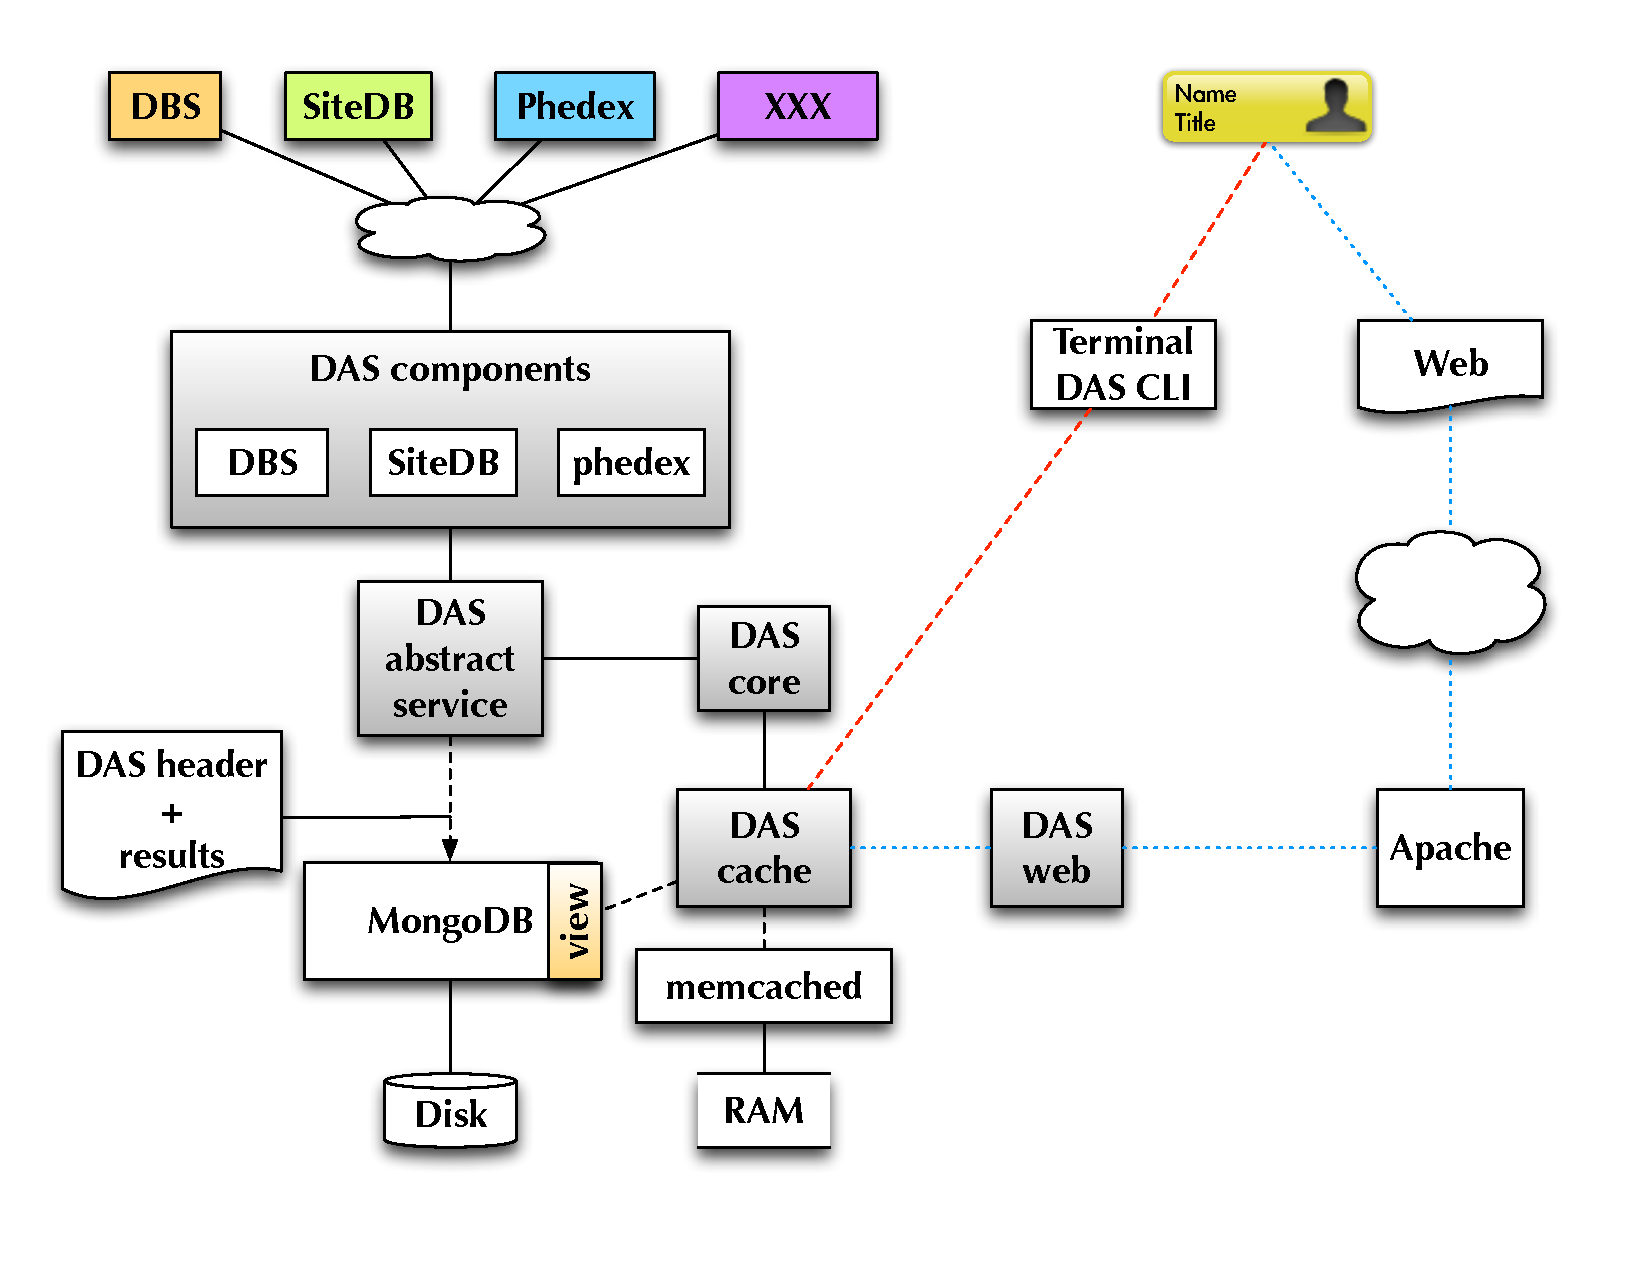
\includegraphics[width=150mm]{DAS_architecture.pdf}
%\caption{
%DAS architecture.
%}
%\label{DAS_arch}
%\end{figure}
\begin{figure}[htb]
\centering
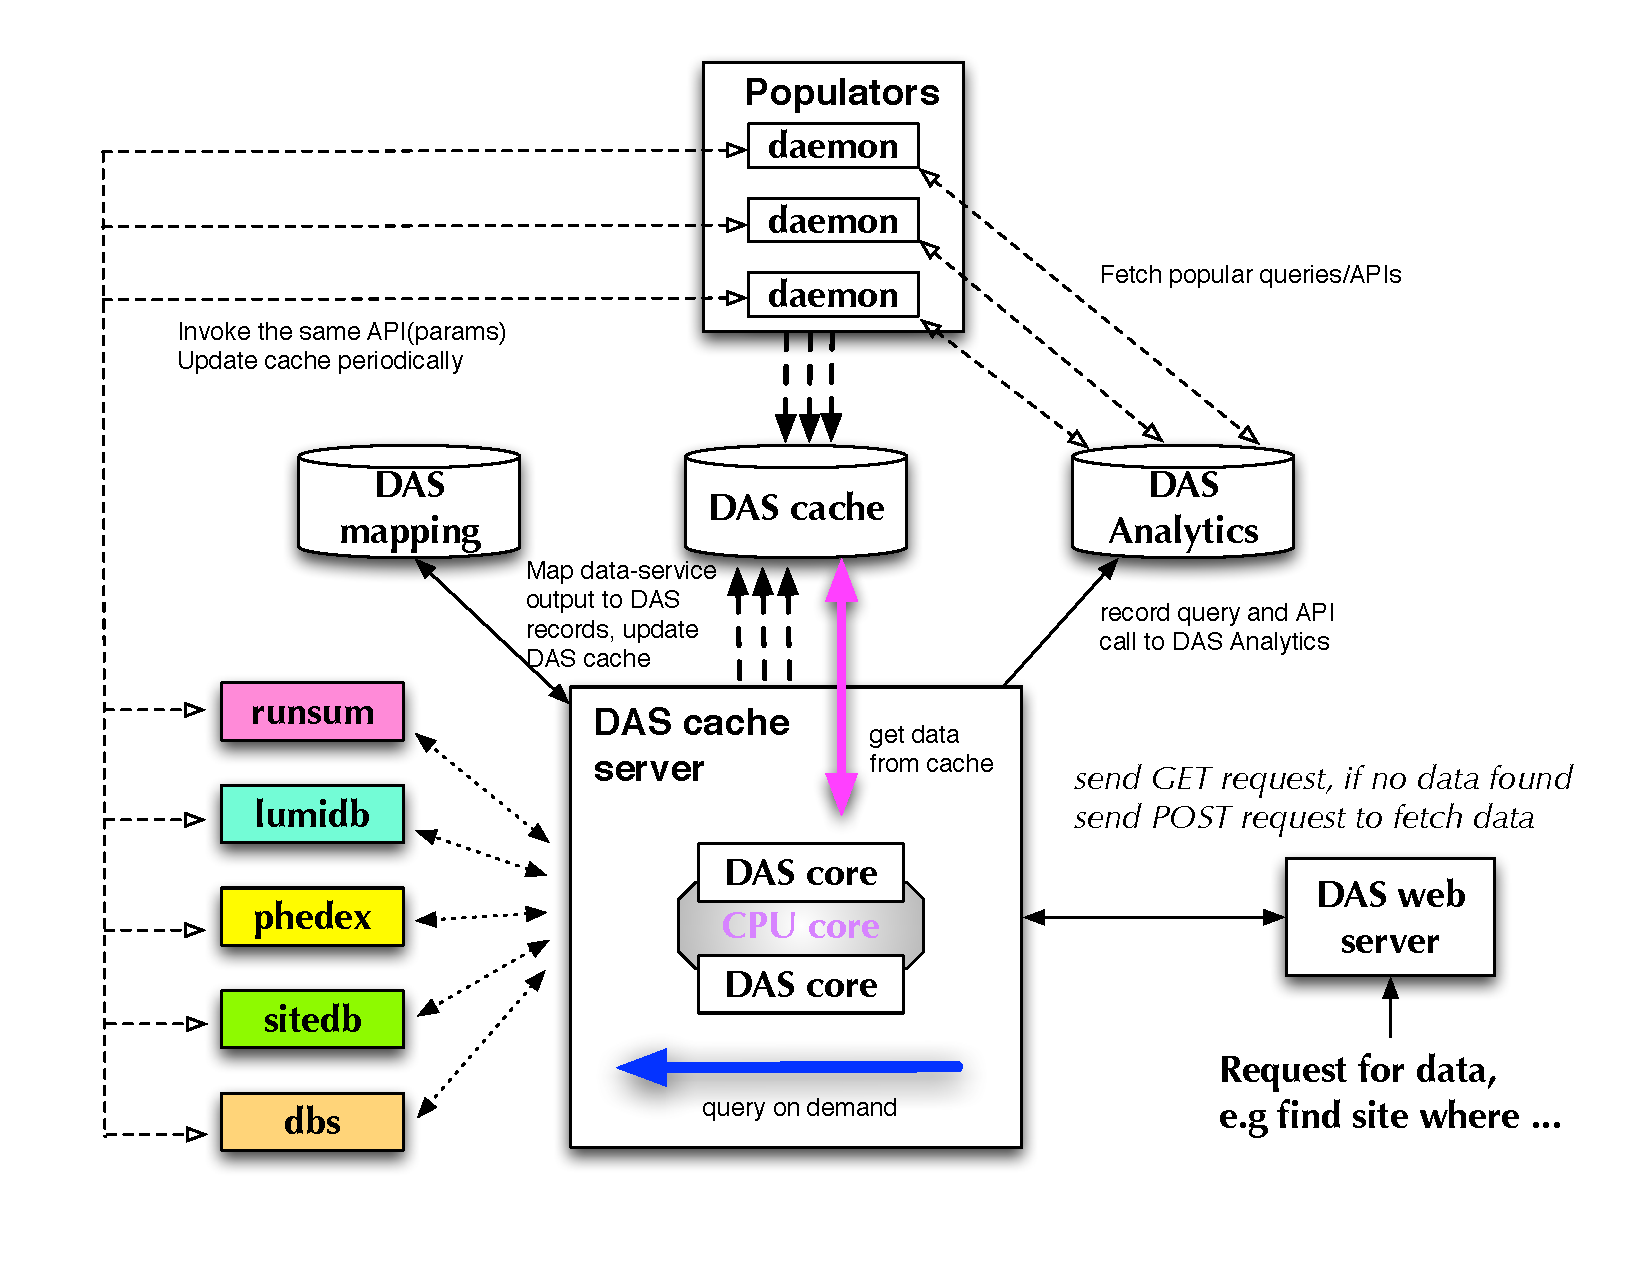
\includegraphics[width=150mm]{DAS_Cache_and_Analytics.pdf}
\caption{
DAS architecture diagram. It consists of DAS cache server, mapping and analytics DBs.
Once query was placed to DAS an associated
data-service API was invoked, triggering DAS cache population. Once data become
available in DAS cache user were able to see the results. This on demand
query retrieval system, where data were retrieved and store into cache from
back-end data service. We use DAS analytics DB to establish cache population
for most common queries by using DAS robots.
}
\label{DAS_cache}
\end{figure}

\noindent
The DAS architecture is shown in Fig. \ref{DAS_cache}. It consists of the
following components:
\begin{itemize}
\item core library with support of pluggable modules for data retrieval;
\item caching layer to store data-service output and aggregated results;
\item request service to handle user requests;
\item mapping DB to keep information about data-service APIs, their
notations and mapping to DAS;
\item analytics DB with query statistics to enable pre-fetching 
strategies.
\end{itemize}

The DAS core communicates with different data-services and retrieve
data on demand. This was done by invoking appropriate data-service APIs
upon user requests. All user queries were written to Analytics DB
for further analysis. The data-service output where re-mapped into
DAS notations and if necessary aggregated inside of DAS cache.
Since we didn't know a-priory what kind of data users will ask, 
what kind of queries they will place against the system and what
level of aggregation will be applied the choice
of RDMS as DAS back-end was problematic\footnote{In addition DAS 
didn't impose any requirements for transactions and persistency of the data.} 
and we look around for other options. Through the analysis of available IT solutions, 
such as file-based and memory caches, 
key-value databases, documented-oriented databases we made our choice in favor 
of the last technology. Among them we evaluated CouchDB \cite{CouchDB} and 
MongoDB \cite{MongoDB}. Both of them provide schema free document
storage, replication and fail-over features, but our choice in favor of 
MongoDB was obvious because its support of dynamic queries, 
full indexies, including on inner objects and embedded arrays,
and auto-sharding. Our prelimiary benchmarks shown that it can sustain
the desired load and size for our meta-data information. We use MongoDB as a back-end 
for the three main components: Mapping, Analytics and DAS cache databases. 

DAS Mapping DB holds mapping between data-service APIs and DAS keys. 
Upon identification of APIs which will participate in DAS activity 
we store to Mapping DB the API name, input parameters, their type and accept 
values as regular expression patterns as well as mapping between data-service 
notations into DAS keys. This allows to map user input query parameters into
data-service API metrics as well as map back data-service output into DAS names.
For instance, the DBS system \cite{DBS}
used {\it logical\_file\_name} notation, while in PhEDEx
\cite{PhEDEx}
the same entity was named as {\it lfn}. Since both of them were referred to
logical file name, we map both notations into DAS key {\it file}.\footnote{We
also deal with physical file names, but still used {\it file} to refer to them in
DAS notation, since simple regular expressions were used to identify {\it file}
meaning from the provided value.}
For each service we provide a mapping from its own data-format (JSON, XML, etc.) into
common data-format used in DAS.\footnote{We used JSON as a DAS data format.}
We also store a mapping between DAS keys and data-service API names to
establish appropriate calls to data-service upon provided DAS query. For example,
when user specifies {\it file} in their DAS query, we invoke DBS listFiles and PhEDEx
fileReplicas APIs. 

The DAS Analytics DB plays special role. It collects information
about user requests placed to the system. Each request was recorded. Upon its
decomposition into set of selection keys and conditions we also record
API name and API input parameters and keep updating their counter for repeated
calls. This allows to keep track of frequency of API calls and establish pre-fetch
strategy for most requested APIs.

The DAS caching system was used to store data-service results and aggregated
information in form of DAS records. As it shown in figure \ref{DAS_cache} 
the DAS cache server updates Analytics DB, requests and retrieve data from DAS cache
and aggregate data over there. The independent set of daemons, DAS robots, are
constantly monitor Analytics DB for most popular requests and pre-fetch most
common data in DAS cache.

Each user request placed to the system was parsed and set of selection
and condition keys were identified. They were mapped into set of
data service APIs and their input parameters. DAS
cache was checked for a similar set of selection and condition
keys which can be placed earlier.\footnote{Since DAS doesn't hold
any data by default we cannot rely on data being present in a cache.
Moreover if we look-up for data first, we cannot tell if it was complete
set since earlier queries may retrieve only portion of the requested data.}
If the superset was found a data were
retrieved from the cache, otherwise a data-service APIs were
invoked and the results were collected and aggregated in DAS cache.

%Now we present overall logic of DAS workflow and details of individual components.
%Upon request to DAS the following steps were executed: 
%\begin{itemize}
%\item parse input DAS query
%\item map provided selection and condition keys into data-service APIs and
%input parameters
%\item look-up similar queries in DAS cache 
%\item invoke data-service APIs
%\item parse output results by mapping output notation into DAS keys
%\item store and aggregate them into DAS raw-cache
%\end{itemize} 

Apart from previous DBS-QL syntax we decided to fully support free text-based queries for end-users.
All of them were transformed into MongoDB query syntax, who was used internally in
DAS core layer. It represents a set of selection keys and conditions as a JSON document.
For example, a query
{\it dataset site=T1\_CH\_CERN}
where transformed into 
{\it \{"fields" : ["dataset"], "spec" : \{"site" : "T1\_CH\_CERN"\}\}}.
Such syntax was perfect fit for us, since it allows us to store all queries
as JSON documents into Analytics DB for further analysis. It is worthwhile to note that
MongoDB query syntax is very reach. It supports advanced queries with 
boolean expressions, conditional operators, regular expression, etc. providing
a real power for our end-users.

\subsection{Data-services and aggregation}
DAS provided a pluggable interface to add new CMS data-services. 
Each data-service plugin consists of its DAS map and individual data parser. 
The data-service DAS map consists of information about data-service APIs,
input and output parameters, data-service
format and their mapping to DAS keys as well as relation to other sub-systems. 
The information was stored into DAS Mapping DB. Below you can see a typical
record of SiteDB \cite{SiteDB} data-service:
\begin{verbatim}
{"api": {"params": {"name": ""}, "name": "CMSNametoSE"}, 
 "api2das": [{"pattern": "re.compile('^T[0-3]_')", 
              "api_param": "name", 
              "das_key": "site"}], 
 "_id": "4ae1f8dfe2194e4581000014", 
 "system": "sitedb", 
 "daskeys": [{"pattern": "re.compile('^T[0-3]_')", 
              "key": "site", 
              "map": "site.name"}]}
\end{verbatim}
It contains information about API name and parameters, mapping between API input
parameter and DAS key, CMS system name and set of DAS keys this API is covering.
We also used regular expression patterns, evaluated by python during run time
execution, to verify provided set of input paremters and DAS keys.

The DAS Mapping DB becomes an authorative
source of information about all data-services participating in DAS and their
relationships. Based on this information we were able to retrieve appropriate data
from different data-services, re-map them into DAS notations and
aggregate them on demand.
For instance, the Data Bookkeeping System (DBS) and data location system (PhEDEx)
provided information about CMS data files. In former case, DBS holds information about
files and their relationship to other physics objects, such as run and luminosity, 
while PhEDEx stores information about the file location, such as sites which
holds copy of the files and details about storage elements.
Upon a user request to find a file, we were able to identify appropriate set of
DBS and PhEDEx APIs, look-up data, re-format their output to DAS notations and
store results into DAS cache.
Once data were retreived from data-services an additional step to aggregate
matched objects in DAS cache were applied. For instance, both data-service outputs 
contained a file name in them. We use it as a common key to merge records in DAS cache.
This merged (aggregated) results represented DAS data objects. Each DAS data
object contains a standard DAS header, which identify look-up time,
request url, input parameters and API method as well as response version, expiration
time and checksum of the output. Here is an example of individual DAS record:
\begin{verbatim}
{"_id": "4ae1e7ffe2194e4243000003", 
 "site":[{"samname": "CERN-PROD", "name": "T1_CH_CERN"}, 
         {"sitename": "CERN", "name": "T1_CH_CERN"}], 
 "das": [{"qhash": ["ed2b73067794d443ed56756d9b94f7bc"], 
          "ctime": 0.95439004898071289, "expire": 1256362175.7692671, 
          "url": "https://cmsweb.cern.ch/sitedb/json/index/CMStoSAMName", 
          "timestamp": 1256318975.7692671, "system": ["sitedb"], 
          "api": ["CMStoSAMName"], "version": "", "selection_keys": []}, 
         {"qhash": ["ed2b73067794d443ed56756d9b94f7bc"], 
          "ctime": 1.2158100605010986, 
          "api": ["CMStoSiteName"], 
          "url": "https://cmsweb.cern.ch/sitedb/json/index/CMStoSiteName", 
          "timestamp": 1256318974.7774379, "system": ["sitedb"], 
          "expire": 1256362174.7774379, "version": "", "selection_keys": []}
        ]
}
\end{verbatim}
It represents aggregated DAS record between two SiteDB APIs, CMStoSAMName and
CMStoSiteName, where API results are merged under {\it site} key. The information
under {\it das} key shows DAS header, which contains sufficient amount of
information about API name, location, execution time and lifetime of the data.
Using this information was valuable contribution in debugging process of
data-services themselves, e.g. identification of not-matched records, 
latency studies, etc.

We used REST model \cite{REST} for all data requests to DAS.
It allows us to share core library and other components during development of 
various DAS clients, e.g. CLI, web interface, robots, etc. and hides
complexity of access to individual data-services and security policies.
For instance, to access on-line Run Summary information we were forced to use
Grid certificates. Instead of propagating user certificate to data-service
the DAS works as a proxy and used host certficiate to serve such requests.

\section{Results\label{Results}}
DAS was deployed to work with the following CMS data-services:
\begin{itemize}
\item DBS \cite{DBS}, Data Bookkeeping System which collect information
about CMS meta-data;
\item PhEDEx \cite{PhEDEx}, Physics Experiment Data Export project which
provides the data placement and the file transfer system for the CMS experiment;
\item SiteDB \cite{SiteDB} is a catalogue of all CMS computing Tiers. 
It records the CMS resources at the site, the resources pledged for the 
future, and it keeps track of CMS personnel at each site, including the 
roles and duties they fulfill in the collaboration;
\item RunSummary DB \cite{RunSummary} collects information about run and triggers
conditions during data-taking;
%\item LumiDB \cite{LumiDB} collects information about Luminosity conditions;
%\item DQ \cite{DQ}, Data Quality data-service which collects information
%about detector conditions during data taking;
%\item Overview \cite{Overview}, collects information about CMS
%transfer rate, etc.;
\item Dashboard \cite{Dashboard} project for LHC experiments aims to 
provide a single entry point to the monitoring data collected from the 
distributed computing systems of the LHC virtual organization.
\end{itemize}
Each data-service has its own scope, size and lifetime. For instance the data
in PhEDEx are transient due to constant migration of CMS data with daily DB size of
around few tens of GBs. The DBS system were divided into dozen of individual instances, 
who has been used by different production teams for various bookkeeping tasks.
Figure \ref{db_size} shows current size of meta-data from aforementioned data-service.
\begin{figure}[htb]
\centering
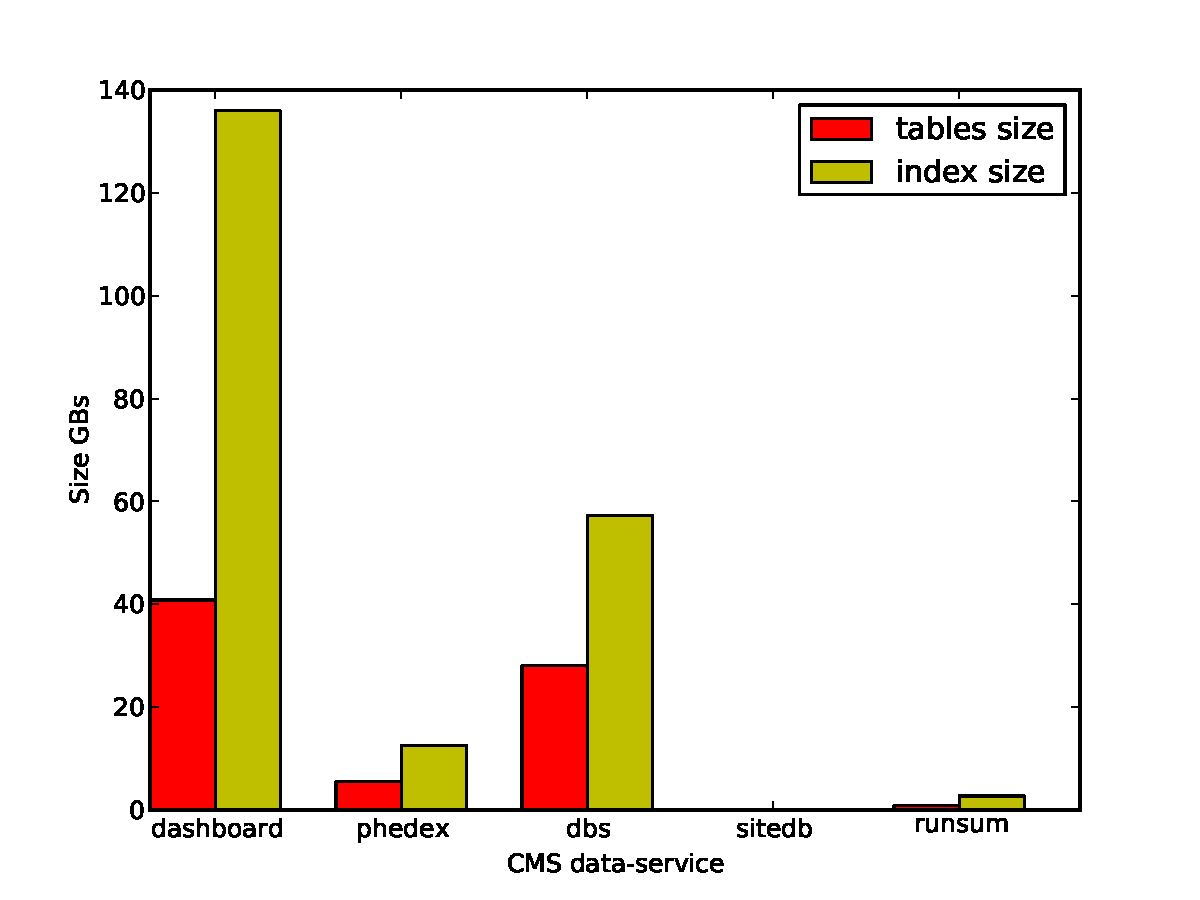
\includegraphics[width=100mm]{db_size.pdf}
\caption{
Database size of CMS data-services participating in DAS in November 2009, before
data taking.
}
\label{db_size}
\end{figure}
%Typical
%size of individual DBS instance was around of fwe GBs, with overall DBS size of
%around of 50 GBs.\footnote{This include table and index sizes.}

At the moment we don't have exact numbers for amount of data which will stored to DAS,
but based on test performed during CRAFT09 \cite{CRAFT09}
exercise we produced 0.3PB of data which
translate into $\sim50$ GB of meta-data stored into DBS system. Therefore
we can anticipate to collect $\sim500$GB of meta-data per year during data-taking period
at LHC.
%In CRAFT09 acquisition era, Tier-0 produced a total of 6.03
%billion events, 330TB in 32 datasets:
%AlCa/Calibration RAW: 926 million events, 29TB
%Physics RAW: 1.24 billion events, 147TB
%PromptReco: 1.24 billion events, 111TB
%Bulk ALCARECO: 2.34 billion events, 11TB
%Express FEVT: 105 million events, 24TB
%Express ALCARECO: 153 million events, 0.99TB
%HLTMON FEVTHLTALL: 31 million events, 7.4TB
%Above event numbers have signicant overlap by design, 
%2.2 billion unique events, including 524 million cosmic muon
%triggers
% 0.3PB - 50GB meta-data in DBS
% 3PB/y - x GB

We did preliminary studies of DAS performance based on information stored
in 2 systems, DBS and PhEDEx. We benchmark time required to collect and 
aggregate block objects information from both system, see Table \ref{DAS_benchmark}.

\begin{table*}[hbt]
\centering
\begin{tabular}{llllll}\hline
\hline

System & Format & Size & Records & Elapsed time & Elapsed time \\
& & & & no cached data & w/ cached data \\
\hline
DAS (DBS) & XML & 187MB & 346820 & 165 sec & 2.53 sec \\
DAS (PhEDEx) & JSON & 164MB & 230035 & 177 sec & 2.42 sec \\
DAS (aggregate) & JSON & 357MB & 348866 & 386 sec & 41.7 sec \\
\hline
\hline
\end{tabular}
\caption{DAS benchmark results. We performed a stress test with 2 CMS system, which
both deliver block object information. The total number of DAS records is calculated
as number of aggregated records and left over from both systems.}
\label{DAS_benchmark}
\end{table*}

We measured elapsed time as the following:
\begin{itemize}
\item[]
{\it
Elapsed time = retrieval time + parsing time + remapping time 
        + cache insertion/indexing time 
        + (aggregation time) + (output creation time)
}
\end{itemize}
Here the {\it retrieval time} is a time required to access data from remote data-services,
{\it parsing time} is a time required to read and parse received data, {\it remapping time}
is a time to convert notations used by data-service to DAS ones for every object
we parse, {\it cache insertion} and {\it indexing time} represents time spend to add objects into
the DAS cache, {\it aggregation time} is required to merge objects into DAS records based
on their common key (block name in this case) and {\it output creation time}
is a time required to write DAS records to disk. Please note that last two
components, {\it aggregation} and {\it output creation time}, were only applied to
final DAS step and not to individual DAS components.

The individual DAS components (DBS and PhEDEx) shown roughly the same performance.
For example, in case of PhEDEx the total time spent in DAS was 177 seconds, where
majority of the time was spent on retrieval, 83 seconds, and parsing, 29 seconds.
The remaining 65 seconds was distributed among remapping, cache insertion, indexing. The
numbers for DBS system were alike. As you can see from Table \ref{DAS_benchmark},
the time spent to read DAS records (last column) from the cache was quite
reasonable, roughly 2.5 seconds from both systems. While final time to
get DAS records on disk was below 42 seconds. This was mostly due to I/O operations.

Based on this results we measured that we can achieve 900 docs/sec for creation of DAS
in a cache and 8500 docs/sec for reading DAS records back, which is suitable for our
needs.\footnote{We've been satisfied with such performance,
even though our measurements shown that it can still be speed up by factor of
10 if we will use C++ DB driver.}

\section{Summary}
We presented new data aggregation service (DAS) developed for CMS High-Energy experiment
at LHC, CERN, Geneva, Switzerland. It was designed to provide caching and
aggregation layer on top of existing relational and non-relation data-service
mostly in real time fashion. All the data were retrieved on demand basis,
while data pre-fetching of most common queries is in our plans. The DAS system 
is under commissioning phase right now and prelimiary performance studies
show it can accommodate needs of CMS experiment as general purpose meta-data
service. The CMS experiment is started to
collect data from November 2009 and we expect to write about PB of data each
year to tape. In addition, the Monte-Carlo samples will be produced at this scale.
Based on test studies performed in CMS, it can translate to the order of
$\sim500$GB of meta-data each year. The DAS should sustain such load and provide
interface as data discovery service in CMS.

\section{Acknowledgments}

This work was supported by the National Science Foundation and Department of Energy of the United States of America. Fermilab is operated by Fermi Research Alliance, LLC under Contract
No. DE-AC02-07CH11359 with the United States Department of Energy.

\section*{References}
\begin{thebibliography}{9}
\bibitem{FedDB}
L. Haas, E. Lin,
``IBM Federated Database Technology'', \\
http://www.ibm.com/developerworks/data/library/techarticle/0203haas/0203haas.html

\bibitem{DBXplorer}
Sanjay Agrawal, Surajit Chaudhuri, Gautam Das: DBXplorer: A System for
Keyword-Based Search over Relational Databases. ICDE 2002: 5-16

\bibitem{QueryAnswer}
Georgia Koutrika, Alkis Simitsis, Yannis E. Ioannidis: Pr\'{e}cis: The Essence of
a Query Answer. ICDE 2006: 69-78

\bibitem{DBS-QL} V. Kuznetsov, D. Riley, A. Afaq, V. Sekhri, Y. Guo, L. Lueking,
``The CMS DBS Query Language'', CHEP 2009

\bibitem{AMI}
Altas AMI web portal:
http://ami.in2p3.fr/opencms/opencms/AMI/www/Tutorial/AMIMediation.html

\bibitem{CMS} CMS Collaboration R. Adolphi et al., The CMS experiment at the CERN LHC, JINST, 0803, S08004 (2008)

\bibitem{CMSDataModel} 
.Grandi, D.Stickland, L.Taylor et al., The CMS Computing Model, CERN-LHCC-2004- 035/G-083 (2004);
A. Fanfani et. al.,
``Distributed Analysis in CMS'', to be published in Journal of Grid Computing.

\bibitem{DBS} A. Afaq, et. al. ``The CMS Dataset Bookkeeping Service'', CHEP 2007 
J.Phys.Conf.Ser, 119, 072001 (2008)

\bibitem{DBS07} A. Dolgert, V. Kuznetsov, C. Jones, D. Riley, 
``A multi-dimensional view on information retrieval of CMS data'', CHEP 2007

\bibitem{DD} https://cmsweb.cern.ch/dbs\_discovery

\bibitem{Arms}
C. R. Arms, W. Y. Arms, ``Mixed Content and Mixed Metadata 
Information Discovery in a Messy World'',
chapter from ``Metadata in Practice'', ALA Editions, 2004

\bibitem{MySQL}
http://www.mysql.com/

\bibitem{CouchDB}
http://couchdb.apache.org/

\bibitem{MongoDB}
http://www.mongodb.org/

\bibitem{REST}
Fielding, Roy Thomas ``Architectural Styles and the Design of 
Network-based Software Architectures'', Doctoral dissertation, 2000,
University of California, Irvine

\bibitem{PhEDEx}
Rehn et. al.,
``PhEDEx high-throughput data transfer management system'', CHEP06, Mumbai, India.
R. Egeland et al., Data transfer infrastructure for CMS data taking, Proceedings of Science,
PoS(ACAT08)033 (2008) ;
L. Tuura et al., Scaling CMS data transfer system for LHC start-up, J.Phys.Conf.Ser, 119, 072030 (2008)

\bibitem{RunSummary}
https://cmswbm.web.cern.ch/cmswbm/cmsdb/servlet/RunSummary

\bibitem{SiteDB}
https://cmsweb.cern.ch/sitedb/

%\bibitem{LumiDB}
%https://twiki.cern.ch/twiki/bin/view/CMS/CMS-DMWM-DBS-Luminosity

%\bibitem{DQ}
%Data-Quality DB reference

%\bibitem{Overview}
%https://cmsweb.cern.ch/overview/

\bibitem{Dashboard}
J. Andreeva, et. al,
``Experiment Dashboard – The Monitoring System for the LHC Experiments'',
GMW’07, June 25, 2007, Monterey, California, USA.

\bibitem{CRAFT09}
https://twiki.cern.ch/twiki/bin/view/CMS/CRAFT09AnalysisInfo

\bibitem{DBSearch}
D. Konopnicki, O. Shmueli,
``Database-Inspired Search'', 
Proc. of the 31st VLDB Conference, 2005.
\end{thebibliography}

\end{document}


